\documentclass[letterpaper,12pt]{article}
\usepackage[margin=14mm,top=18mm,bottom=17mm,headheight=14pt]{geometry}
\pdfmapfile{+cm.map}\pdfmapfile{+cmextra.map}
\usepackage{tikz,fancyhdr,amsmath,amssymb}
\usetikzlibrary{arrows.meta,patterns}
\pagestyle{fancy}\fancyhf{}\renewcommand{\headrulewidth}{0pt}
\fancyhead[L]{\small Week 47 / Gentle-step landscapes / Grades 4--5}
\fancyfoot[L]{\small Bellingham Math Circle / Week 47 / F47-45-v4}
\fancyfoot[R]{\small\thepage}
\setlength{\parindent}{0pt}\setlength{\parskip}{0pt}
\begin{document}
\noindent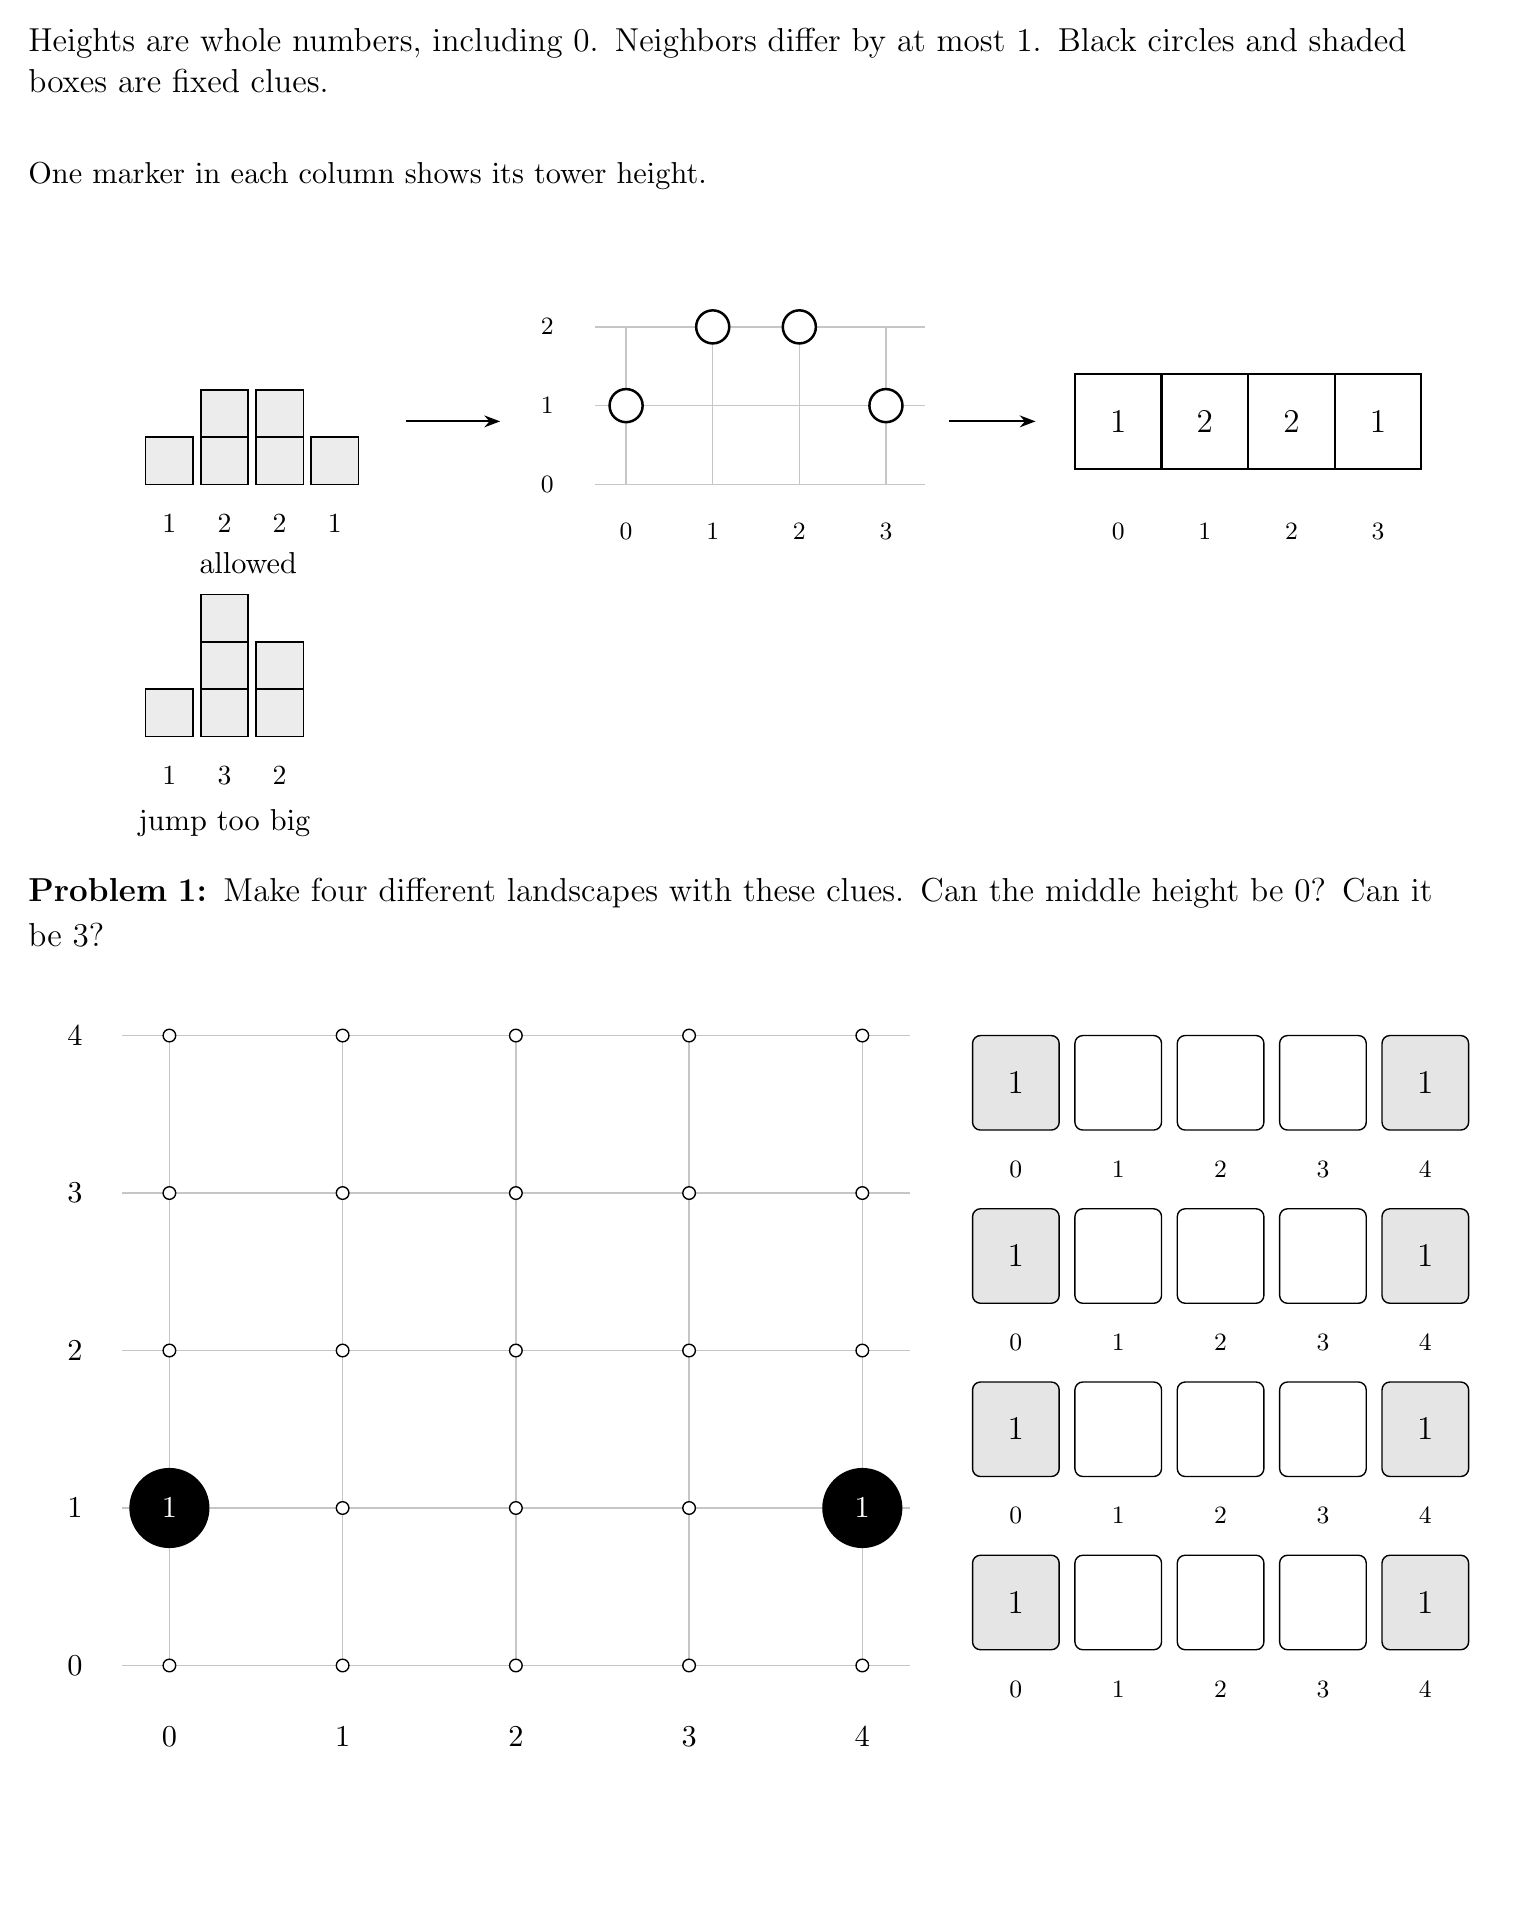
\begin{tikzpicture}[x=1mm,y=-1mm,line width=.5pt]
\path[use as bounding box] (0,0) rectangle (185,235);
\node[anchor=north west,inner sep=0pt,text width=180mm,font=\fontsize{12}{15}\selectfont] at (0,0) {Heights are whole numbers, including 0. Neighbors differ by at most 1. Black circles and shaded boxes are fixed clues.};
\node[anchor=north west,inner sep=0pt,text width=180mm,font=\fontsize{11}{14}\selectfont] at (0,17) {One marker in each column shows its tower height.};
\draw[fill=gray!15] (15,52) rectangle ++(6,6);
\node[anchor=center,inner sep=1pt,font=\fontsize{10}{12}\selectfont] at (18.0,63) {1};
\draw[fill=gray!15] (22,52) rectangle ++(6,6);
\draw[fill=gray!15] (22,46) rectangle ++(6,6);
\node[anchor=center,inner sep=1pt,font=\fontsize{10}{12}\selectfont] at (25.0,63) {2};
\draw[fill=gray!15] (29,52) rectangle ++(6,6);
\draw[fill=gray!15] (29,46) rectangle ++(6,6);
\node[anchor=center,inner sep=1pt,font=\fontsize{10}{12}\selectfont] at (32.0,63) {2};
\draw[fill=gray!15] (36,52) rectangle ++(6,6);
\node[anchor=center,inner sep=1pt,font=\fontsize{10}{12}\selectfont] at (39.0,63) {1};
\node[anchor=center,inner sep=1pt,font=\fontsize{11}{13}\selectfont] at (28,68) {allowed};
\draw[gray!45] (72,58) -- (114,58);
\node[anchor=center,inner sep=1pt,font=\fontsize{9}{11}\selectfont] at (66,58) {0};
\draw[gray!45] (72,48) -- (114,48);
\node[anchor=center,inner sep=1pt,font=\fontsize{9}{11}\selectfont] at (66,48) {1};
\draw[gray!45] (72,38) -- (114,38);
\node[anchor=center,inner sep=1pt,font=\fontsize{9}{11}\selectfont] at (66,38) {2};
\draw[gray!45] (76,38) -- (76,58);
\draw[fill=white,line width=.9pt] (76,48) circle (2.1);
\node[anchor=center,inner sep=1pt,font=\fontsize{9}{11}\selectfont] at (76,64) {0};
\draw[gray!45] (87,38) -- (87,58);
\draw[fill=white,line width=.9pt] (87,38) circle (2.1);
\node[anchor=center,inner sep=1pt,font=\fontsize{9}{11}\selectfont] at (87,64) {1};
\draw[gray!45] (98,38) -- (98,58);
\draw[fill=white,line width=.9pt] (98,38) circle (2.1);
\node[anchor=center,inner sep=1pt,font=\fontsize{9}{11}\selectfont] at (98,64) {2};
\draw[gray!45] (109,38) -- (109,58);
\draw[fill=white,line width=.9pt] (109,48) circle (2.1);
\node[anchor=center,inner sep=1pt,font=\fontsize{9}{11}\selectfont] at (109,64) {3};
\draw[-{Stealth[length=2mm]},line width=.8pt] (48,50) -- (60,50);
\draw[-{Stealth[length=2mm]},line width=.8pt] (117,50) -- (128,50);
\draw[line width=.8pt] (133,44) rectangle ++(44,12);
\node[anchor=center,inner sep=1pt,font=\fontsize{13}{15}\selectfont] at (138.5,50) {1};
\node[anchor=center,inner sep=1pt,font=\fontsize{9}{11}\selectfont] at (138.5,64) {0};
\draw[line width=.8pt] (144,44) -- (144,56);
\node[anchor=center,inner sep=1pt,font=\fontsize{13}{15}\selectfont] at (149.5,50) {2};
\node[anchor=center,inner sep=1pt,font=\fontsize{9}{11}\selectfont] at (149.5,64) {1};
\draw[line width=.8pt] (155,44) -- (155,56);
\node[anchor=center,inner sep=1pt,font=\fontsize{13}{15}\selectfont] at (160.5,50) {2};
\node[anchor=center,inner sep=1pt,font=\fontsize{9}{11}\selectfont] at (160.5,64) {2};
\draw[line width=.8pt] (166,44) -- (166,56);
\node[anchor=center,inner sep=1pt,font=\fontsize{13}{15}\selectfont] at (171.5,50) {1};
\node[anchor=center,inner sep=1pt,font=\fontsize{9}{11}\selectfont] at (171.5,64) {3};
\draw[fill=gray!15] (15,84) rectangle ++(6,6);
\node[anchor=center,inner sep=1pt,font=\fontsize{10}{12}\selectfont] at (18.0,95) {1};
\draw[fill=gray!15] (22,84) rectangle ++(6,6);
\draw[fill=gray!15] (22,78) rectangle ++(6,6);
\draw[fill=gray!15] (22,72) rectangle ++(6,6);
\node[anchor=center,inner sep=1pt,font=\fontsize{10}{12}\selectfont] at (25.0,95) {3};
\draw[fill=gray!15] (29,84) rectangle ++(6,6);
\draw[fill=gray!15] (29,78) rectangle ++(6,6);
\node[anchor=center,inner sep=1pt,font=\fontsize{10}{12}\selectfont] at (32.0,95) {2};
\node[anchor=center,inner sep=1pt,font=\fontsize{11}{13}\selectfont] at (25,101) {jump too big};
\node[anchor=north west,inner sep=0pt,text width=180mm,font=\fontsize{13}{16}\selectfont] at (0,108) {\textbf{Problem 1:} Make four different landscapes with these clues. Can the middle height be 0? Can it be 3?};
\draw[gray!45] (12,208) -- (112,208);
\node[anchor=center,inner sep=1pt,font=\fontsize{11}{13}\selectfont] at (6,208) {0};
\draw[gray!45] (12,188) -- (112,188);
\node[anchor=center,inner sep=1pt,font=\fontsize{11}{13}\selectfont] at (6,188) {1};
\draw[gray!45] (12,168) -- (112,168);
\node[anchor=center,inner sep=1pt,font=\fontsize{11}{13}\selectfont] at (6,168) {2};
\draw[gray!45] (12,148) -- (112,148);
\node[anchor=center,inner sep=1pt,font=\fontsize{11}{13}\selectfont] at (6,148) {3};
\draw[gray!45] (12,128) -- (112,128);
\node[anchor=center,inner sep=1pt,font=\fontsize{11}{13}\selectfont] at (6,128) {4};
\draw[gray!45] (18,128) -- (18,208);
\draw[fill=white] (18,208) circle (0.8);
\draw[fill=white] (18,188) circle (0.8);
\draw[fill=white] (18,168) circle (0.8);
\draw[fill=white] (18,148) circle (0.8);
\draw[fill=white] (18,128) circle (0.8);
\node[anchor=center,inner sep=1pt,font=\fontsize{11}{13}\selectfont] at (18,217) {0};
\draw[fill=black] (18,188) circle (5);
\node[anchor=center,inner sep=1pt,font=\fontsize{11}{13}\selectfont] at (18,188) {\color{white}1};
\draw[gray!45] (40,128) -- (40,208);
\draw[fill=white] (40,208) circle (0.8);
\draw[fill=white] (40,188) circle (0.8);
\draw[fill=white] (40,168) circle (0.8);
\draw[fill=white] (40,148) circle (0.8);
\draw[fill=white] (40,128) circle (0.8);
\node[anchor=center,inner sep=1pt,font=\fontsize{11}{13}\selectfont] at (40,217) {1};
\draw[gray!45] (62,128) -- (62,208);
\draw[fill=white] (62,208) circle (0.8);
\draw[fill=white] (62,188) circle (0.8);
\draw[fill=white] (62,168) circle (0.8);
\draw[fill=white] (62,148) circle (0.8);
\draw[fill=white] (62,128) circle (0.8);
\node[anchor=center,inner sep=1pt,font=\fontsize{11}{13}\selectfont] at (62,217) {2};
\draw[gray!45] (84,128) -- (84,208);
\draw[fill=white] (84,208) circle (0.8);
\draw[fill=white] (84,188) circle (0.8);
\draw[fill=white] (84,168) circle (0.8);
\draw[fill=white] (84,148) circle (0.8);
\draw[fill=white] (84,128) circle (0.8);
\node[anchor=center,inner sep=1pt,font=\fontsize{11}{13}\selectfont] at (84,217) {3};
\draw[gray!45] (106,128) -- (106,208);
\draw[fill=white] (106,208) circle (0.8);
\draw[fill=white] (106,188) circle (0.8);
\draw[fill=white] (106,168) circle (0.8);
\draw[fill=white] (106,148) circle (0.8);
\draw[fill=white] (106,128) circle (0.8);
\node[anchor=center,inner sep=1pt,font=\fontsize{11}{13}\selectfont] at (106,217) {4};
\draw[fill=black] (106,188) circle (5);
\node[anchor=center,inner sep=1pt,font=\fontsize{11}{13}\selectfont] at (106,188) {\color{white}1};
\draw[rounded corners=1mm,fill=gray!20] (120,128) rectangle ++(11,12);
\node[anchor=center,inner sep=1pt,font=\fontsize{13}{15}\selectfont] at (125.5,134) {1};
\node[anchor=center,inner sep=1pt,font=\fontsize{9}{11}\selectfont] at (125.5,145) {0};
\draw[rounded corners=1mm] (133,128) rectangle ++(11,12);
\node[anchor=center,inner sep=1pt,font=\fontsize{13}{15}\selectfont] at (138.5,134) {};
\node[anchor=center,inner sep=1pt,font=\fontsize{9}{11}\selectfont] at (138.5,145) {1};
\draw[rounded corners=1mm] (146,128) rectangle ++(11,12);
\node[anchor=center,inner sep=1pt,font=\fontsize{13}{15}\selectfont] at (151.5,134) {};
\node[anchor=center,inner sep=1pt,font=\fontsize{9}{11}\selectfont] at (151.5,145) {2};
\draw[rounded corners=1mm] (159,128) rectangle ++(11,12);
\node[anchor=center,inner sep=1pt,font=\fontsize{13}{15}\selectfont] at (164.5,134) {};
\node[anchor=center,inner sep=1pt,font=\fontsize{9}{11}\selectfont] at (164.5,145) {3};
\draw[rounded corners=1mm,fill=gray!20] (172,128) rectangle ++(11,12);
\node[anchor=center,inner sep=1pt,font=\fontsize{13}{15}\selectfont] at (177.5,134) {1};
\node[anchor=center,inner sep=1pt,font=\fontsize{9}{11}\selectfont] at (177.5,145) {4};
\draw[rounded corners=1mm,fill=gray!20] (120,150) rectangle ++(11,12);
\node[anchor=center,inner sep=1pt,font=\fontsize{13}{15}\selectfont] at (125.5,156) {1};
\node[anchor=center,inner sep=1pt,font=\fontsize{9}{11}\selectfont] at (125.5,167) {0};
\draw[rounded corners=1mm] (133,150) rectangle ++(11,12);
\node[anchor=center,inner sep=1pt,font=\fontsize{13}{15}\selectfont] at (138.5,156) {};
\node[anchor=center,inner sep=1pt,font=\fontsize{9}{11}\selectfont] at (138.5,167) {1};
\draw[rounded corners=1mm] (146,150) rectangle ++(11,12);
\node[anchor=center,inner sep=1pt,font=\fontsize{13}{15}\selectfont] at (151.5,156) {};
\node[anchor=center,inner sep=1pt,font=\fontsize{9}{11}\selectfont] at (151.5,167) {2};
\draw[rounded corners=1mm] (159,150) rectangle ++(11,12);
\node[anchor=center,inner sep=1pt,font=\fontsize{13}{15}\selectfont] at (164.5,156) {};
\node[anchor=center,inner sep=1pt,font=\fontsize{9}{11}\selectfont] at (164.5,167) {3};
\draw[rounded corners=1mm,fill=gray!20] (172,150) rectangle ++(11,12);
\node[anchor=center,inner sep=1pt,font=\fontsize{13}{15}\selectfont] at (177.5,156) {1};
\node[anchor=center,inner sep=1pt,font=\fontsize{9}{11}\selectfont] at (177.5,167) {4};
\draw[rounded corners=1mm,fill=gray!20] (120,172) rectangle ++(11,12);
\node[anchor=center,inner sep=1pt,font=\fontsize{13}{15}\selectfont] at (125.5,178) {1};
\node[anchor=center,inner sep=1pt,font=\fontsize{9}{11}\selectfont] at (125.5,189) {0};
\draw[rounded corners=1mm] (133,172) rectangle ++(11,12);
\node[anchor=center,inner sep=1pt,font=\fontsize{13}{15}\selectfont] at (138.5,178) {};
\node[anchor=center,inner sep=1pt,font=\fontsize{9}{11}\selectfont] at (138.5,189) {1};
\draw[rounded corners=1mm] (146,172) rectangle ++(11,12);
\node[anchor=center,inner sep=1pt,font=\fontsize{13}{15}\selectfont] at (151.5,178) {};
\node[anchor=center,inner sep=1pt,font=\fontsize{9}{11}\selectfont] at (151.5,189) {2};
\draw[rounded corners=1mm] (159,172) rectangle ++(11,12);
\node[anchor=center,inner sep=1pt,font=\fontsize{13}{15}\selectfont] at (164.5,178) {};
\node[anchor=center,inner sep=1pt,font=\fontsize{9}{11}\selectfont] at (164.5,189) {3};
\draw[rounded corners=1mm,fill=gray!20] (172,172) rectangle ++(11,12);
\node[anchor=center,inner sep=1pt,font=\fontsize{13}{15}\selectfont] at (177.5,178) {1};
\node[anchor=center,inner sep=1pt,font=\fontsize{9}{11}\selectfont] at (177.5,189) {4};
\draw[rounded corners=1mm,fill=gray!20] (120,194) rectangle ++(11,12);
\node[anchor=center,inner sep=1pt,font=\fontsize{13}{15}\selectfont] at (125.5,200) {1};
\node[anchor=center,inner sep=1pt,font=\fontsize{9}{11}\selectfont] at (125.5,211) {0};
\draw[rounded corners=1mm] (133,194) rectangle ++(11,12);
\node[anchor=center,inner sep=1pt,font=\fontsize{13}{15}\selectfont] at (138.5,200) {};
\node[anchor=center,inner sep=1pt,font=\fontsize{9}{11}\selectfont] at (138.5,211) {1};
\draw[rounded corners=1mm] (146,194) rectangle ++(11,12);
\node[anchor=center,inner sep=1pt,font=\fontsize{13}{15}\selectfont] at (151.5,200) {};
\node[anchor=center,inner sep=1pt,font=\fontsize{9}{11}\selectfont] at (151.5,211) {2};
\draw[rounded corners=1mm] (159,194) rectangle ++(11,12);
\node[anchor=center,inner sep=1pt,font=\fontsize{13}{15}\selectfont] at (164.5,200) {};
\node[anchor=center,inner sep=1pt,font=\fontsize{9}{11}\selectfont] at (164.5,211) {3};
\draw[rounded corners=1mm,fill=gray!20] (172,194) rectangle ++(11,12);
\node[anchor=center,inner sep=1pt,font=\fontsize{13}{15}\selectfont] at (177.5,200) {1};
\node[anchor=center,inner sep=1pt,font=\fontsize{9}{11}\selectfont] at (177.5,211) {4};
\end{tikzpicture}
\newpage
\noindent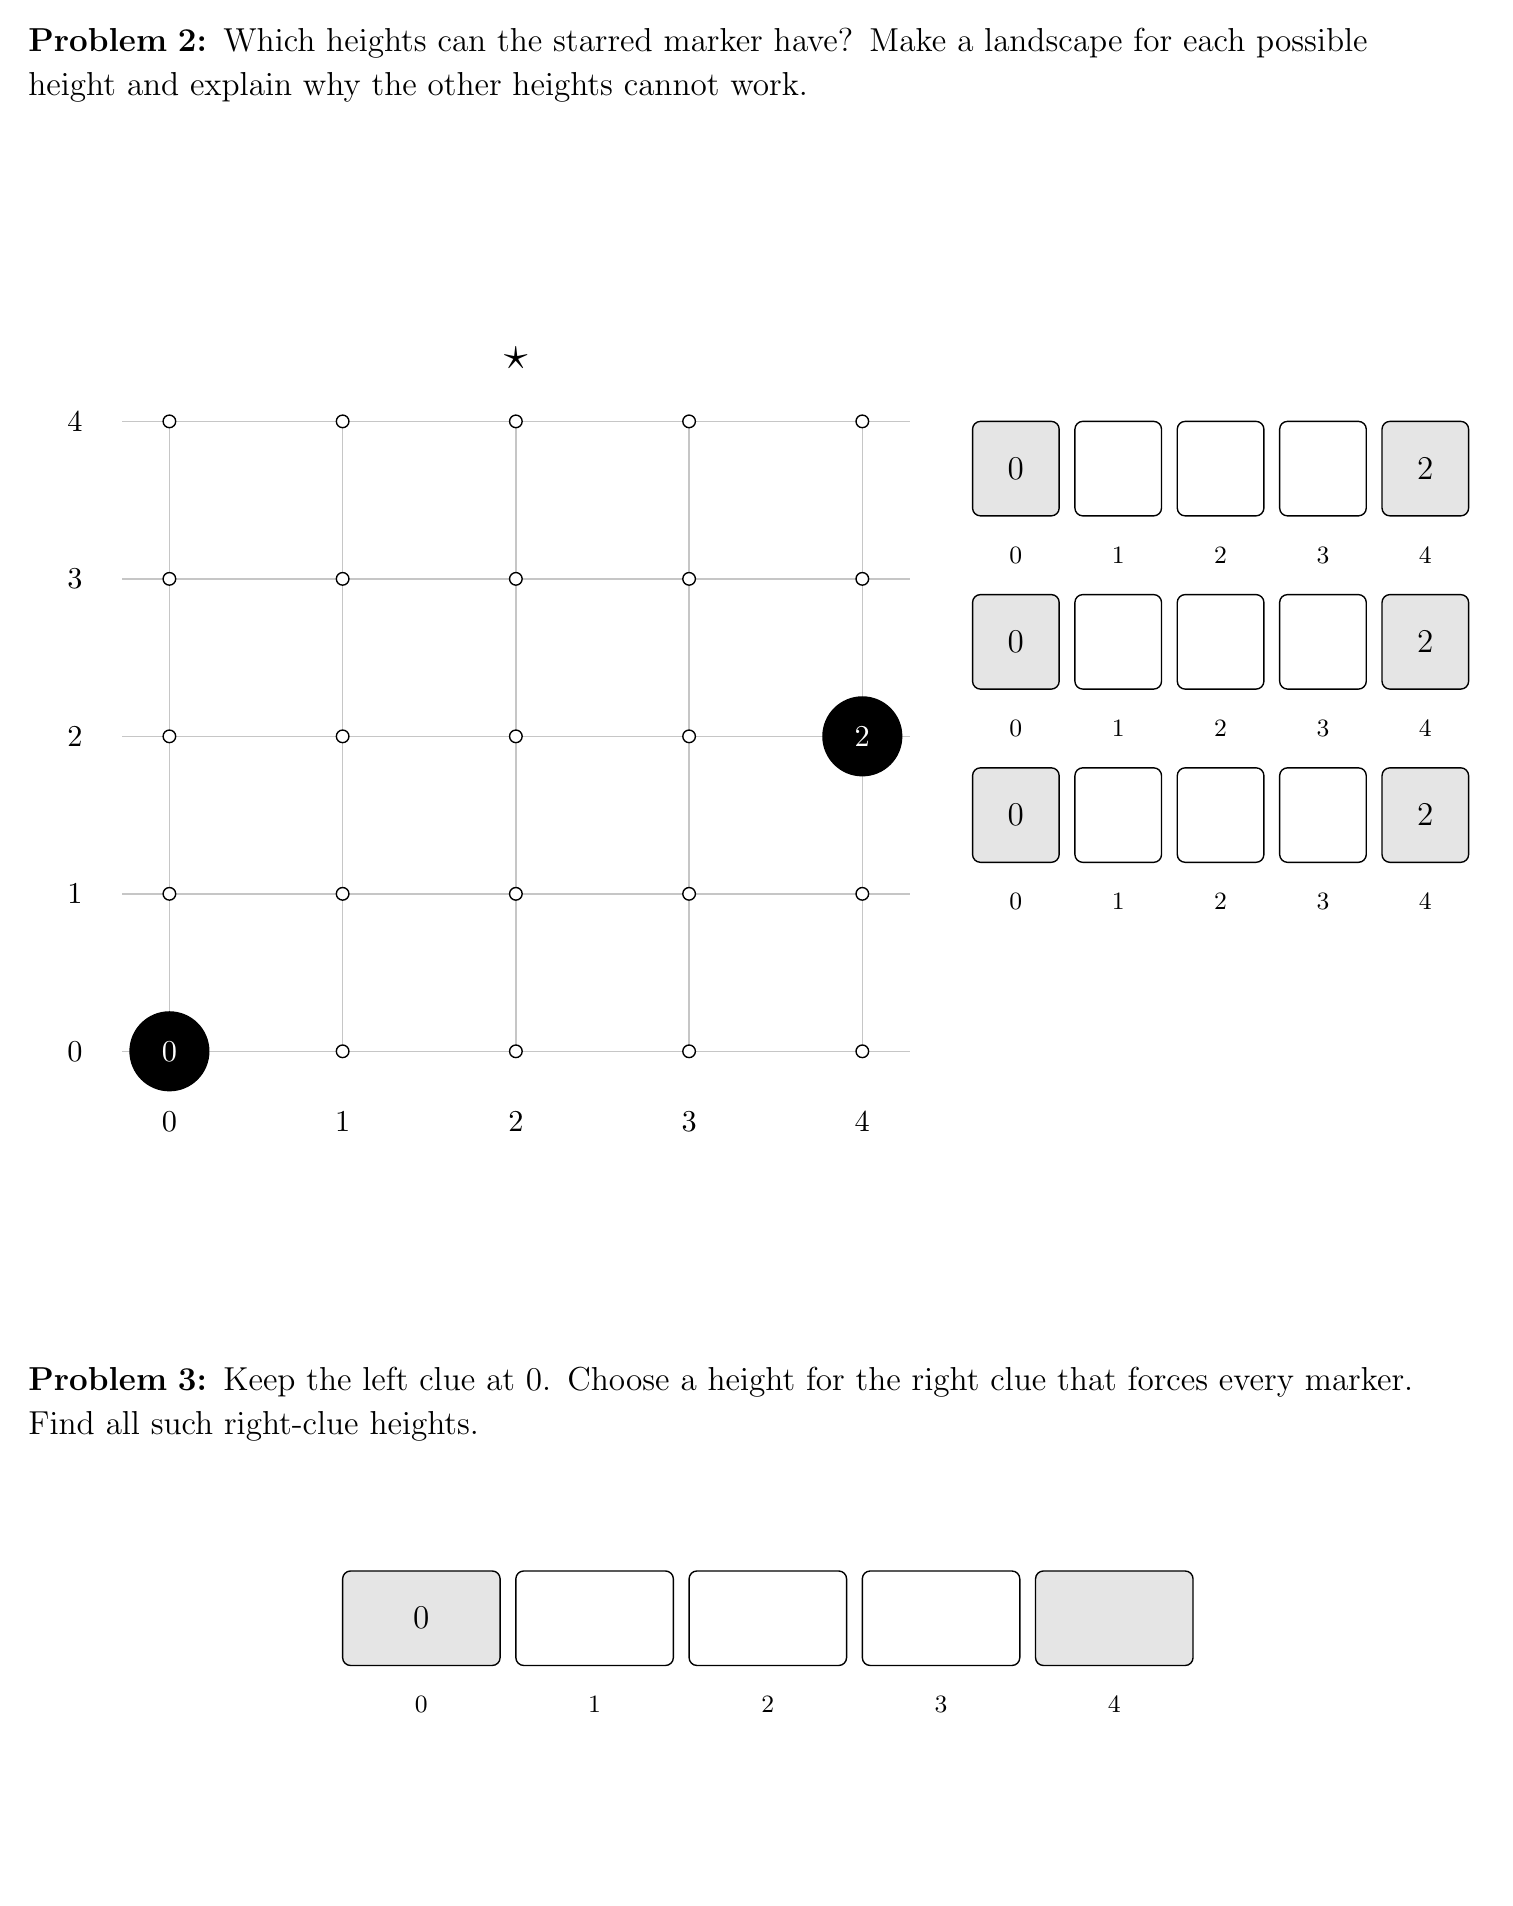
\begin{tikzpicture}[x=1mm,y=-1mm,line width=.5pt]
\path[use as bounding box] (0,0) rectangle (185,235);
\node[anchor=north west,inner sep=0pt,text width=180mm,font=\fontsize{13}{16}\selectfont] at (0,0) {\textbf{Problem 2:} Which heights can the starred marker have? Make a landscape for each possible height and explain why the other heights cannot work.};
\draw[gray!45] (12,130) -- (112,130);
\node[anchor=center,inner sep=1pt,font=\fontsize{11}{13}\selectfont] at (6,130) {0};
\draw[gray!45] (12,110) -- (112,110);
\node[anchor=center,inner sep=1pt,font=\fontsize{11}{13}\selectfont] at (6,110) {1};
\draw[gray!45] (12,90) -- (112,90);
\node[anchor=center,inner sep=1pt,font=\fontsize{11}{13}\selectfont] at (6,90) {2};
\draw[gray!45] (12,70) -- (112,70);
\node[anchor=center,inner sep=1pt,font=\fontsize{11}{13}\selectfont] at (6,70) {3};
\draw[gray!45] (12,50) -- (112,50);
\node[anchor=center,inner sep=1pt,font=\fontsize{11}{13}\selectfont] at (6,50) {4};
\draw[gray!45] (18,50) -- (18,130);
\draw[fill=white] (18,130) circle (0.8);
\draw[fill=white] (18,110) circle (0.8);
\draw[fill=white] (18,90) circle (0.8);
\draw[fill=white] (18,70) circle (0.8);
\draw[fill=white] (18,50) circle (0.8);
\node[anchor=center,inner sep=1pt,font=\fontsize{11}{13}\selectfont] at (18,139) {0};
\draw[fill=black] (18,130) circle (5);
\node[anchor=center,inner sep=1pt,font=\fontsize{11}{13}\selectfont] at (18,130) {\color{white}0};
\draw[gray!45] (40,50) -- (40,130);
\draw[fill=white] (40,130) circle (0.8);
\draw[fill=white] (40,110) circle (0.8);
\draw[fill=white] (40,90) circle (0.8);
\draw[fill=white] (40,70) circle (0.8);
\draw[fill=white] (40,50) circle (0.8);
\node[anchor=center,inner sep=1pt,font=\fontsize{11}{13}\selectfont] at (40,139) {1};
\draw[gray!45] (62,50) -- (62,130);
\draw[fill=white] (62,130) circle (0.8);
\draw[fill=white] (62,110) circle (0.8);
\draw[fill=white] (62,90) circle (0.8);
\draw[fill=white] (62,70) circle (0.8);
\draw[fill=white] (62,50) circle (0.8);
\node[anchor=center,inner sep=1pt,font=\fontsize{11}{13}\selectfont] at (62,139) {2};
\node[anchor=center,inner sep=1pt,font=\fontsize{16}{18}\selectfont] at (62,42) {$\star$};
\draw[gray!45] (84,50) -- (84,130);
\draw[fill=white] (84,130) circle (0.8);
\draw[fill=white] (84,110) circle (0.8);
\draw[fill=white] (84,90) circle (0.8);
\draw[fill=white] (84,70) circle (0.8);
\draw[fill=white] (84,50) circle (0.8);
\node[anchor=center,inner sep=1pt,font=\fontsize{11}{13}\selectfont] at (84,139) {3};
\draw[gray!45] (106,50) -- (106,130);
\draw[fill=white] (106,130) circle (0.8);
\draw[fill=white] (106,110) circle (0.8);
\draw[fill=white] (106,90) circle (0.8);
\draw[fill=white] (106,70) circle (0.8);
\draw[fill=white] (106,50) circle (0.8);
\node[anchor=center,inner sep=1pt,font=\fontsize{11}{13}\selectfont] at (106,139) {4};
\draw[fill=black] (106,90) circle (5);
\node[anchor=center,inner sep=1pt,font=\fontsize{11}{13}\selectfont] at (106,90) {\color{white}2};
\draw[rounded corners=1mm,fill=gray!20] (120,50) rectangle ++(11,12);
\node[anchor=center,inner sep=1pt,font=\fontsize{13}{15}\selectfont] at (125.5,56) {0};
\node[anchor=center,inner sep=1pt,font=\fontsize{9}{11}\selectfont] at (125.5,67) {0};
\draw[rounded corners=1mm] (133,50) rectangle ++(11,12);
\node[anchor=center,inner sep=1pt,font=\fontsize{13}{15}\selectfont] at (138.5,56) {};
\node[anchor=center,inner sep=1pt,font=\fontsize{9}{11}\selectfont] at (138.5,67) {1};
\draw[rounded corners=1mm] (146,50) rectangle ++(11,12);
\node[anchor=center,inner sep=1pt,font=\fontsize{13}{15}\selectfont] at (151.5,56) {};
\node[anchor=center,inner sep=1pt,font=\fontsize{9}{11}\selectfont] at (151.5,67) {2};
\draw[rounded corners=1mm] (159,50) rectangle ++(11,12);
\node[anchor=center,inner sep=1pt,font=\fontsize{13}{15}\selectfont] at (164.5,56) {};
\node[anchor=center,inner sep=1pt,font=\fontsize{9}{11}\selectfont] at (164.5,67) {3};
\draw[rounded corners=1mm,fill=gray!20] (172,50) rectangle ++(11,12);
\node[anchor=center,inner sep=1pt,font=\fontsize{13}{15}\selectfont] at (177.5,56) {2};
\node[anchor=center,inner sep=1pt,font=\fontsize{9}{11}\selectfont] at (177.5,67) {4};
\draw[rounded corners=1mm,fill=gray!20] (120,72) rectangle ++(11,12);
\node[anchor=center,inner sep=1pt,font=\fontsize{13}{15}\selectfont] at (125.5,78) {0};
\node[anchor=center,inner sep=1pt,font=\fontsize{9}{11}\selectfont] at (125.5,89) {0};
\draw[rounded corners=1mm] (133,72) rectangle ++(11,12);
\node[anchor=center,inner sep=1pt,font=\fontsize{13}{15}\selectfont] at (138.5,78) {};
\node[anchor=center,inner sep=1pt,font=\fontsize{9}{11}\selectfont] at (138.5,89) {1};
\draw[rounded corners=1mm] (146,72) rectangle ++(11,12);
\node[anchor=center,inner sep=1pt,font=\fontsize{13}{15}\selectfont] at (151.5,78) {};
\node[anchor=center,inner sep=1pt,font=\fontsize{9}{11}\selectfont] at (151.5,89) {2};
\draw[rounded corners=1mm] (159,72) rectangle ++(11,12);
\node[anchor=center,inner sep=1pt,font=\fontsize{13}{15}\selectfont] at (164.5,78) {};
\node[anchor=center,inner sep=1pt,font=\fontsize{9}{11}\selectfont] at (164.5,89) {3};
\draw[rounded corners=1mm,fill=gray!20] (172,72) rectangle ++(11,12);
\node[anchor=center,inner sep=1pt,font=\fontsize{13}{15}\selectfont] at (177.5,78) {2};
\node[anchor=center,inner sep=1pt,font=\fontsize{9}{11}\selectfont] at (177.5,89) {4};
\draw[rounded corners=1mm,fill=gray!20] (120,94) rectangle ++(11,12);
\node[anchor=center,inner sep=1pt,font=\fontsize{13}{15}\selectfont] at (125.5,100) {0};
\node[anchor=center,inner sep=1pt,font=\fontsize{9}{11}\selectfont] at (125.5,111) {0};
\draw[rounded corners=1mm] (133,94) rectangle ++(11,12);
\node[anchor=center,inner sep=1pt,font=\fontsize{13}{15}\selectfont] at (138.5,100) {};
\node[anchor=center,inner sep=1pt,font=\fontsize{9}{11}\selectfont] at (138.5,111) {1};
\draw[rounded corners=1mm] (146,94) rectangle ++(11,12);
\node[anchor=center,inner sep=1pt,font=\fontsize{13}{15}\selectfont] at (151.5,100) {};
\node[anchor=center,inner sep=1pt,font=\fontsize{9}{11}\selectfont] at (151.5,111) {2};
\draw[rounded corners=1mm] (159,94) rectangle ++(11,12);
\node[anchor=center,inner sep=1pt,font=\fontsize{13}{15}\selectfont] at (164.5,100) {};
\node[anchor=center,inner sep=1pt,font=\fontsize{9}{11}\selectfont] at (164.5,111) {3};
\draw[rounded corners=1mm,fill=gray!20] (172,94) rectangle ++(11,12);
\node[anchor=center,inner sep=1pt,font=\fontsize{13}{15}\selectfont] at (177.5,100) {2};
\node[anchor=center,inner sep=1pt,font=\fontsize{9}{11}\selectfont] at (177.5,111) {4};
\node[anchor=north west,inner sep=0pt,text width=180mm,font=\fontsize{13}{16}\selectfont] at (0,170) {\textbf{Problem 3:} Keep the left clue at 0. Choose a height for the right clue that forces every marker. Find all such right-clue heights.};
\draw[rounded corners=1mm,fill=gray!20] (40,196) rectangle ++(20,12);
\node[anchor=center,inner sep=1pt,font=\fontsize{13}{15}\selectfont] at (50.0,202) {0};
\node[anchor=center,inner sep=1pt,font=\fontsize{9}{11}\selectfont] at (50.0,213) {0};
\draw[rounded corners=1mm] (62,196) rectangle ++(20,12);
\node[anchor=center,inner sep=1pt,font=\fontsize{13}{15}\selectfont] at (72.0,202) {};
\node[anchor=center,inner sep=1pt,font=\fontsize{9}{11}\selectfont] at (72.0,213) {1};
\draw[rounded corners=1mm] (84,196) rectangle ++(20,12);
\node[anchor=center,inner sep=1pt,font=\fontsize{13}{15}\selectfont] at (94.0,202) {};
\node[anchor=center,inner sep=1pt,font=\fontsize{9}{11}\selectfont] at (94.0,213) {2};
\draw[rounded corners=1mm] (106,196) rectangle ++(20,12);
\node[anchor=center,inner sep=1pt,font=\fontsize{13}{15}\selectfont] at (116.0,202) {};
\node[anchor=center,inner sep=1pt,font=\fontsize{9}{11}\selectfont] at (116.0,213) {3};
\draw[rounded corners=1mm,fill=gray!20] (128,196) rectangle ++(20,12);
\node[anchor=center,inner sep=1pt,font=\fontsize{13}{15}\selectfont] at (138.0,202) {};
\node[anchor=center,inner sep=1pt,font=\fontsize{9}{11}\selectfont] at (138.0,213) {4};
\end{tikzpicture}
\newpage
\noindent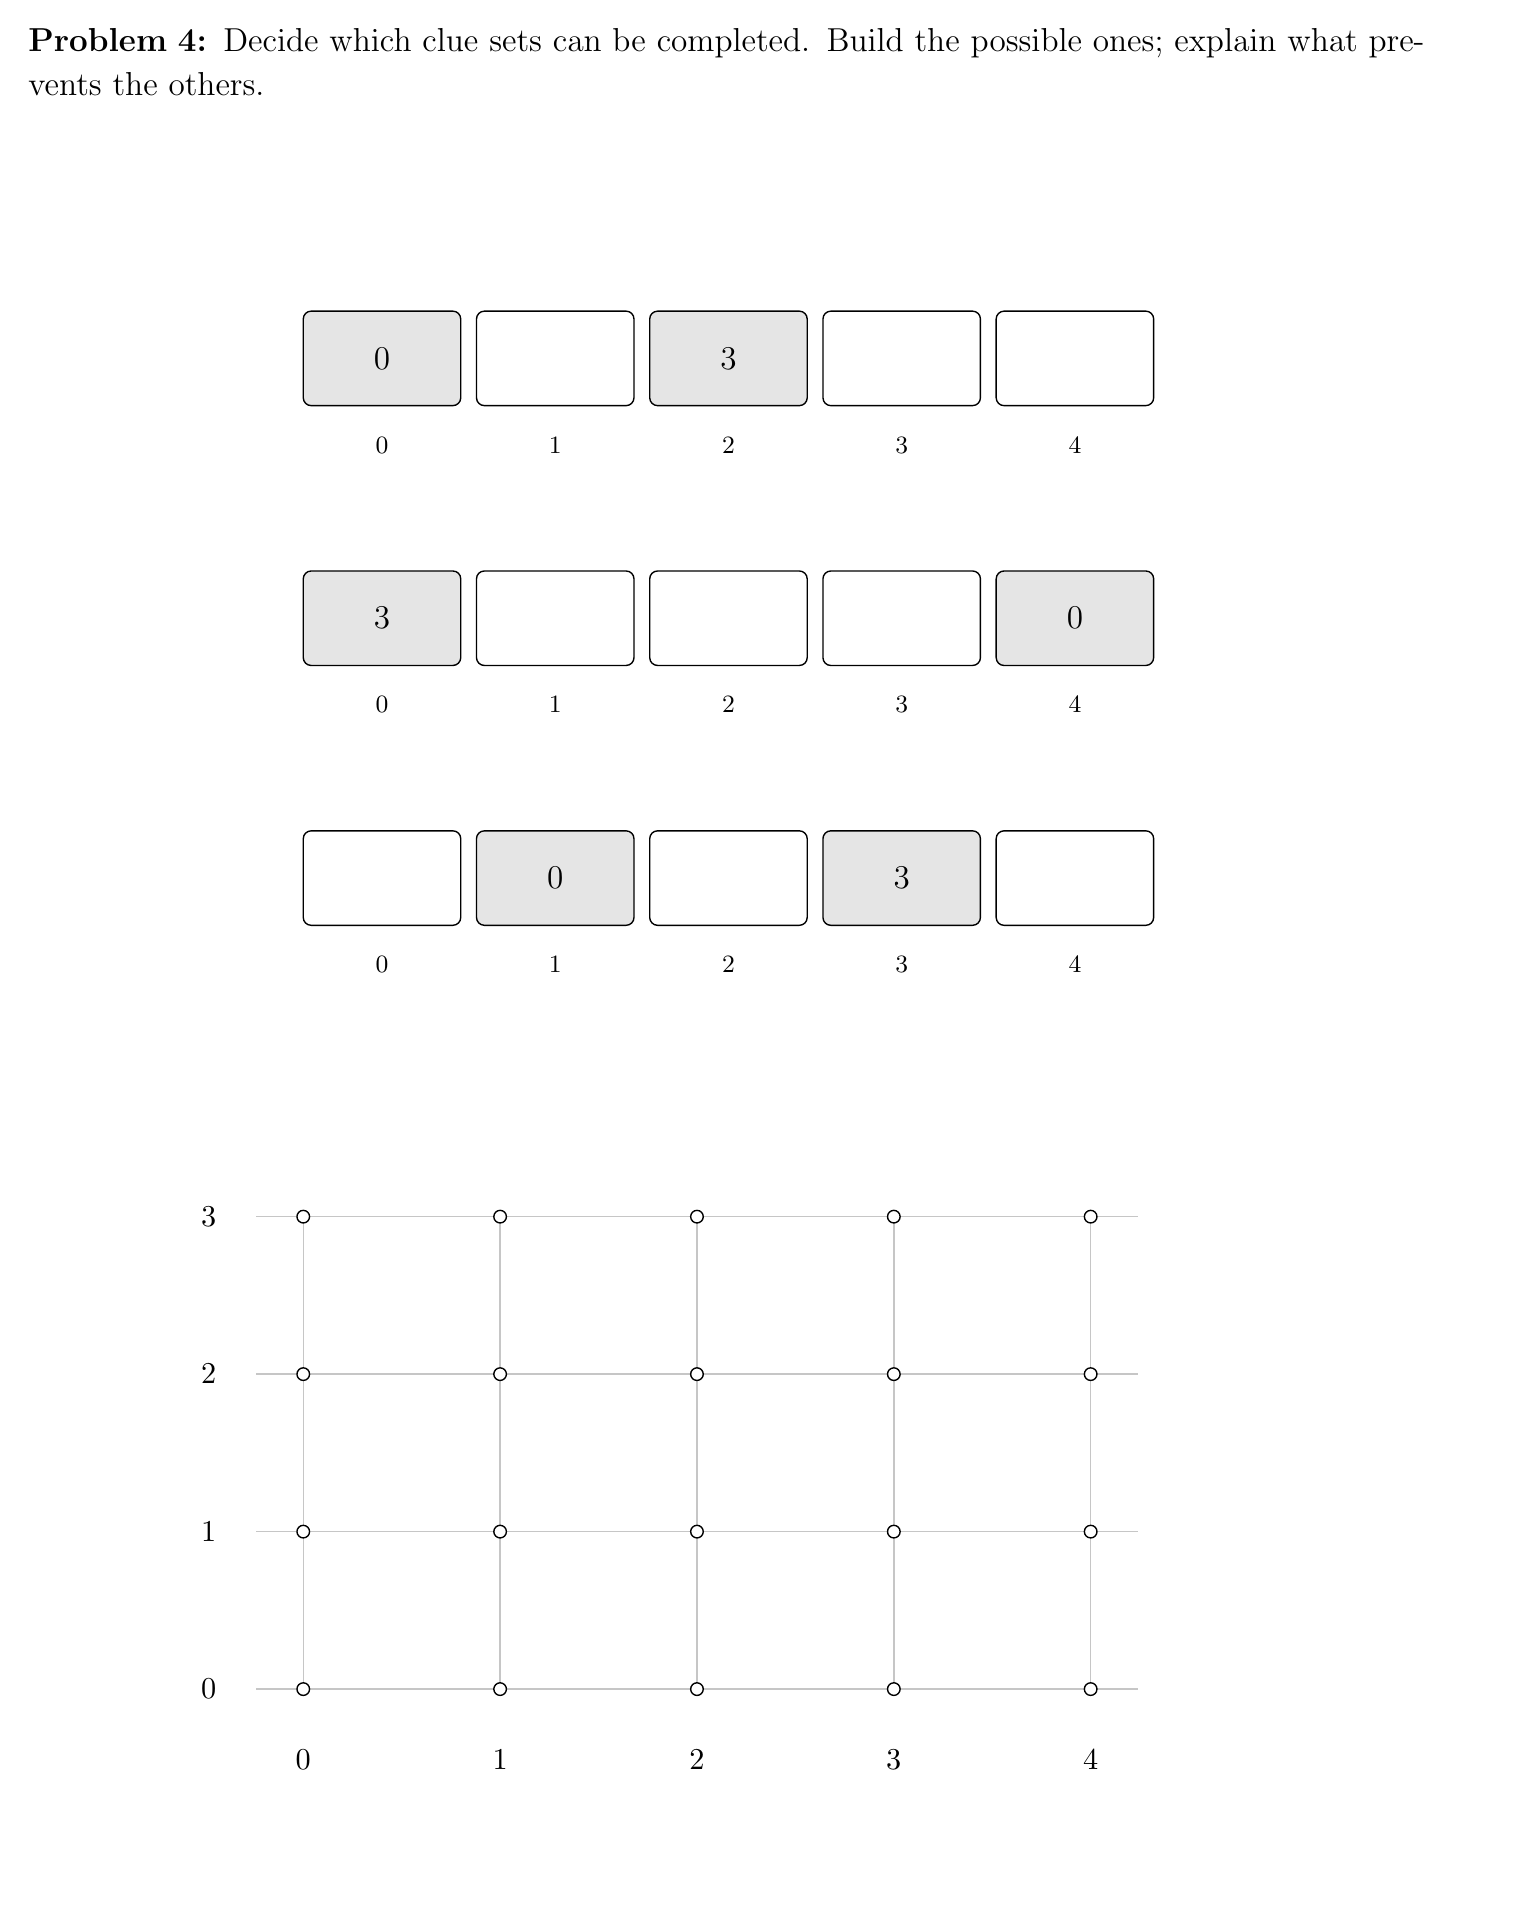
\begin{tikzpicture}[x=1mm,y=-1mm,line width=.5pt]
\path[use as bounding box] (0,0) rectangle (185,235);
\node[anchor=north west,inner sep=0pt,text width=180mm,font=\fontsize{13}{16}\selectfont] at (0,0) {\textbf{Problem 4:} Decide which clue sets can be completed. Build the possible ones; explain what prevents the others.};
\draw[rounded corners=1mm,fill=gray!20] (35,36) rectangle ++(20,12);
\node[anchor=center,inner sep=1pt,font=\fontsize{13}{15}\selectfont] at (45.0,42) {0};
\node[anchor=center,inner sep=1pt,font=\fontsize{9}{11}\selectfont] at (45.0,53) {0};
\draw[rounded corners=1mm] (57,36) rectangle ++(20,12);
\node[anchor=center,inner sep=1pt,font=\fontsize{13}{15}\selectfont] at (67.0,42) {};
\node[anchor=center,inner sep=1pt,font=\fontsize{9}{11}\selectfont] at (67.0,53) {1};
\draw[rounded corners=1mm,fill=gray!20] (79,36) rectangle ++(20,12);
\node[anchor=center,inner sep=1pt,font=\fontsize{13}{15}\selectfont] at (89.0,42) {3};
\node[anchor=center,inner sep=1pt,font=\fontsize{9}{11}\selectfont] at (89.0,53) {2};
\draw[rounded corners=1mm] (101,36) rectangle ++(20,12);
\node[anchor=center,inner sep=1pt,font=\fontsize{13}{15}\selectfont] at (111.0,42) {};
\node[anchor=center,inner sep=1pt,font=\fontsize{9}{11}\selectfont] at (111.0,53) {3};
\draw[rounded corners=1mm] (123,36) rectangle ++(20,12);
\node[anchor=center,inner sep=1pt,font=\fontsize{13}{15}\selectfont] at (133.0,42) {};
\node[anchor=center,inner sep=1pt,font=\fontsize{9}{11}\selectfont] at (133.0,53) {4};
\draw[rounded corners=1mm,fill=gray!20] (35,69) rectangle ++(20,12);
\node[anchor=center,inner sep=1pt,font=\fontsize{13}{15}\selectfont] at (45.0,75) {3};
\node[anchor=center,inner sep=1pt,font=\fontsize{9}{11}\selectfont] at (45.0,86) {0};
\draw[rounded corners=1mm] (57,69) rectangle ++(20,12);
\node[anchor=center,inner sep=1pt,font=\fontsize{13}{15}\selectfont] at (67.0,75) {};
\node[anchor=center,inner sep=1pt,font=\fontsize{9}{11}\selectfont] at (67.0,86) {1};
\draw[rounded corners=1mm] (79,69) rectangle ++(20,12);
\node[anchor=center,inner sep=1pt,font=\fontsize{13}{15}\selectfont] at (89.0,75) {};
\node[anchor=center,inner sep=1pt,font=\fontsize{9}{11}\selectfont] at (89.0,86) {2};
\draw[rounded corners=1mm] (101,69) rectangle ++(20,12);
\node[anchor=center,inner sep=1pt,font=\fontsize{13}{15}\selectfont] at (111.0,75) {};
\node[anchor=center,inner sep=1pt,font=\fontsize{9}{11}\selectfont] at (111.0,86) {3};
\draw[rounded corners=1mm,fill=gray!20] (123,69) rectangle ++(20,12);
\node[anchor=center,inner sep=1pt,font=\fontsize{13}{15}\selectfont] at (133.0,75) {0};
\node[anchor=center,inner sep=1pt,font=\fontsize{9}{11}\selectfont] at (133.0,86) {4};
\draw[rounded corners=1mm] (35,102) rectangle ++(20,12);
\node[anchor=center,inner sep=1pt,font=\fontsize{13}{15}\selectfont] at (45.0,108) {};
\node[anchor=center,inner sep=1pt,font=\fontsize{9}{11}\selectfont] at (45.0,119) {0};
\draw[rounded corners=1mm,fill=gray!20] (57,102) rectangle ++(20,12);
\node[anchor=center,inner sep=1pt,font=\fontsize{13}{15}\selectfont] at (67.0,108) {0};
\node[anchor=center,inner sep=1pt,font=\fontsize{9}{11}\selectfont] at (67.0,119) {1};
\draw[rounded corners=1mm] (79,102) rectangle ++(20,12);
\node[anchor=center,inner sep=1pt,font=\fontsize{13}{15}\selectfont] at (89.0,108) {};
\node[anchor=center,inner sep=1pt,font=\fontsize{9}{11}\selectfont] at (89.0,119) {2};
\draw[rounded corners=1mm,fill=gray!20] (101,102) rectangle ++(20,12);
\node[anchor=center,inner sep=1pt,font=\fontsize{13}{15}\selectfont] at (111.0,108) {3};
\node[anchor=center,inner sep=1pt,font=\fontsize{9}{11}\selectfont] at (111.0,119) {3};
\draw[rounded corners=1mm] (123,102) rectangle ++(20,12);
\node[anchor=center,inner sep=1pt,font=\fontsize{13}{15}\selectfont] at (133.0,108) {};
\node[anchor=center,inner sep=1pt,font=\fontsize{9}{11}\selectfont] at (133.0,119) {4};
\draw[gray!45] (29,211) -- (141,211);
\node[anchor=center,inner sep=1pt,font=\fontsize{11}{13}\selectfont] at (23,211) {0};
\draw[gray!45] (29,191) -- (141,191);
\node[anchor=center,inner sep=1pt,font=\fontsize{11}{13}\selectfont] at (23,191) {1};
\draw[gray!45] (29,171) -- (141,171);
\node[anchor=center,inner sep=1pt,font=\fontsize{11}{13}\selectfont] at (23,171) {2};
\draw[gray!45] (29,151) -- (141,151);
\node[anchor=center,inner sep=1pt,font=\fontsize{11}{13}\selectfont] at (23,151) {3};
\draw[gray!45] (35,151) -- (35,211);
\draw[fill=white] (35,211) circle (0.8);
\draw[fill=white] (35,191) circle (0.8);
\draw[fill=white] (35,171) circle (0.8);
\draw[fill=white] (35,151) circle (0.8);
\node[anchor=center,inner sep=1pt,font=\fontsize{11}{13}\selectfont] at (35,220) {0};
\draw[gray!45] (60,151) -- (60,211);
\draw[fill=white] (60,211) circle (0.8);
\draw[fill=white] (60,191) circle (0.8);
\draw[fill=white] (60,171) circle (0.8);
\draw[fill=white] (60,151) circle (0.8);
\node[anchor=center,inner sep=1pt,font=\fontsize{11}{13}\selectfont] at (60,220) {1};
\draw[gray!45] (85,151) -- (85,211);
\draw[fill=white] (85,211) circle (0.8);
\draw[fill=white] (85,191) circle (0.8);
\draw[fill=white] (85,171) circle (0.8);
\draw[fill=white] (85,151) circle (0.8);
\node[anchor=center,inner sep=1pt,font=\fontsize{11}{13}\selectfont] at (85,220) {2};
\draw[gray!45] (110,151) -- (110,211);
\draw[fill=white] (110,211) circle (0.8);
\draw[fill=white] (110,191) circle (0.8);
\draw[fill=white] (110,171) circle (0.8);
\draw[fill=white] (110,151) circle (0.8);
\node[anchor=center,inner sep=1pt,font=\fontsize{11}{13}\selectfont] at (110,220) {3};
\draw[gray!45] (135,151) -- (135,211);
\draw[fill=white] (135,211) circle (0.8);
\draw[fill=white] (135,191) circle (0.8);
\draw[fill=white] (135,171) circle (0.8);
\draw[fill=white] (135,151) circle (0.8);
\node[anchor=center,inner sep=1pt,font=\fontsize{11}{13}\selectfont] at (135,220) {4};
\end{tikzpicture}
\newpage
\noindent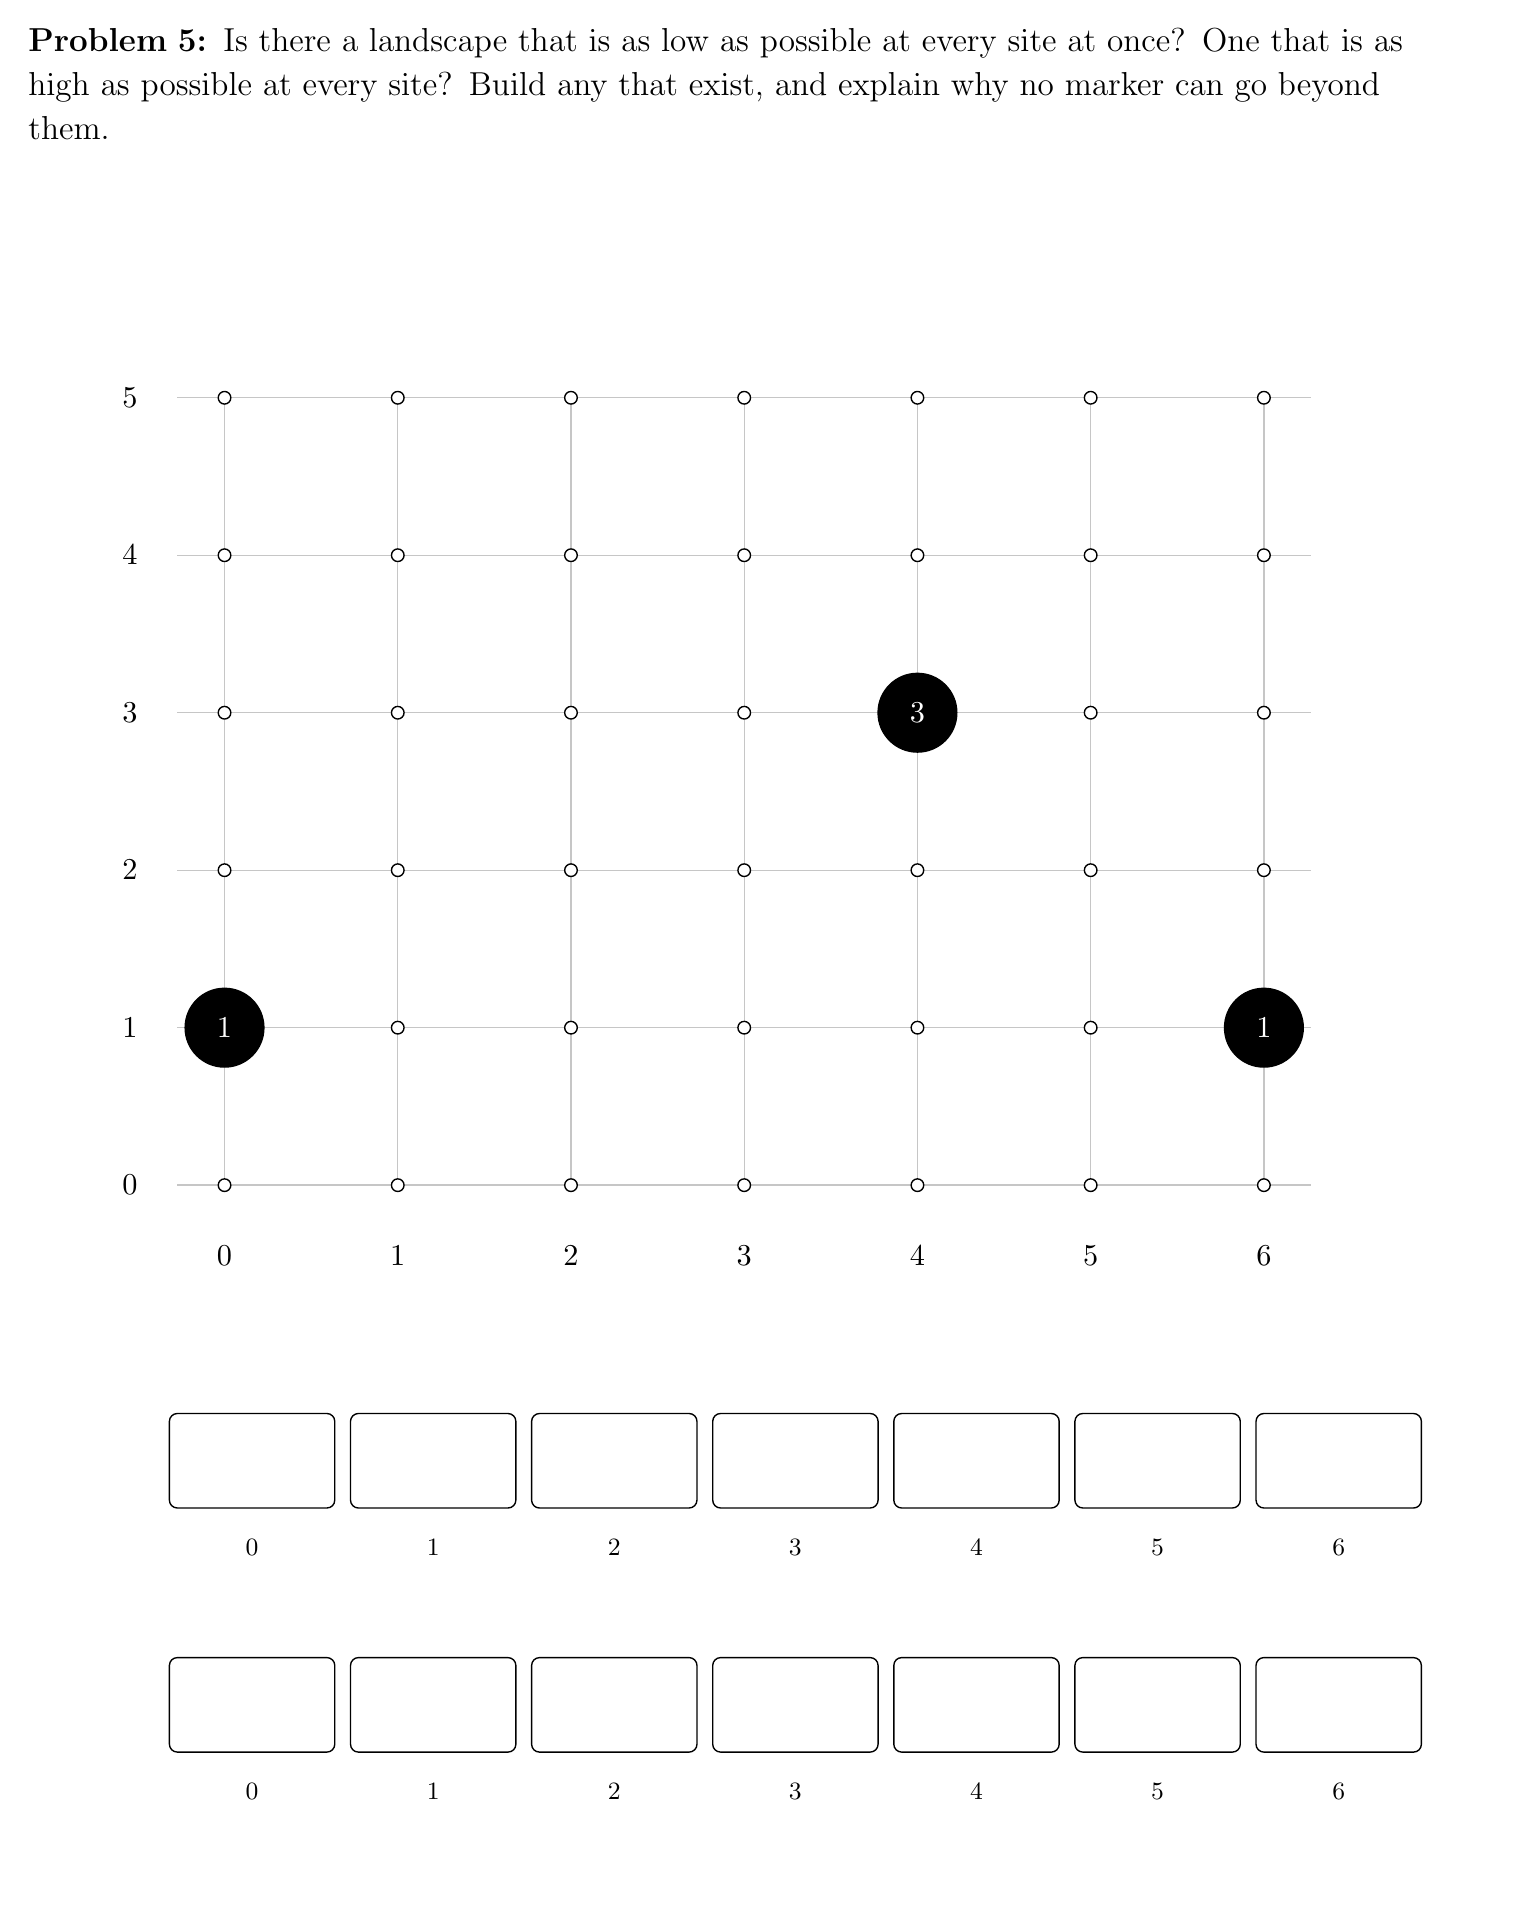
\begin{tikzpicture}[x=1mm,y=-1mm,line width=.5pt]
\path[use as bounding box] (0,0) rectangle (185,235);
\node[anchor=north west,inner sep=0pt,text width=180mm,font=\fontsize{13}{16}\selectfont] at (0,0) {\textbf{Problem 5:} Is there a landscape that is as low as possible at every site at once? One that is as high as possible at every site? Build any that exist, and explain why no marker can go beyond them.};
\draw[gray!45] (19,147) -- (163,147);
\node[anchor=center,inner sep=1pt,font=\fontsize{11}{13}\selectfont] at (13,147) {0};
\draw[gray!45] (19,127) -- (163,127);
\node[anchor=center,inner sep=1pt,font=\fontsize{11}{13}\selectfont] at (13,127) {1};
\draw[gray!45] (19,107) -- (163,107);
\node[anchor=center,inner sep=1pt,font=\fontsize{11}{13}\selectfont] at (13,107) {2};
\draw[gray!45] (19,87) -- (163,87);
\node[anchor=center,inner sep=1pt,font=\fontsize{11}{13}\selectfont] at (13,87) {3};
\draw[gray!45] (19,67) -- (163,67);
\node[anchor=center,inner sep=1pt,font=\fontsize{11}{13}\selectfont] at (13,67) {4};
\draw[gray!45] (19,47) -- (163,47);
\node[anchor=center,inner sep=1pt,font=\fontsize{11}{13}\selectfont] at (13,47) {5};
\draw[gray!45] (25,47) -- (25,147);
\draw[fill=white] (25,147) circle (0.8);
\draw[fill=white] (25,127) circle (0.8);
\draw[fill=white] (25,107) circle (0.8);
\draw[fill=white] (25,87) circle (0.8);
\draw[fill=white] (25,67) circle (0.8);
\draw[fill=white] (25,47) circle (0.8);
\node[anchor=center,inner sep=1pt,font=\fontsize{11}{13}\selectfont] at (25,156) {0};
\draw[fill=black] (25,127) circle (5);
\node[anchor=center,inner sep=1pt,font=\fontsize{11}{13}\selectfont] at (25,127) {\color{white}1};
\draw[gray!45] (47,47) -- (47,147);
\draw[fill=white] (47,147) circle (0.8);
\draw[fill=white] (47,127) circle (0.8);
\draw[fill=white] (47,107) circle (0.8);
\draw[fill=white] (47,87) circle (0.8);
\draw[fill=white] (47,67) circle (0.8);
\draw[fill=white] (47,47) circle (0.8);
\node[anchor=center,inner sep=1pt,font=\fontsize{11}{13}\selectfont] at (47,156) {1};
\draw[gray!45] (69,47) -- (69,147);
\draw[fill=white] (69,147) circle (0.8);
\draw[fill=white] (69,127) circle (0.8);
\draw[fill=white] (69,107) circle (0.8);
\draw[fill=white] (69,87) circle (0.8);
\draw[fill=white] (69,67) circle (0.8);
\draw[fill=white] (69,47) circle (0.8);
\node[anchor=center,inner sep=1pt,font=\fontsize{11}{13}\selectfont] at (69,156) {2};
\draw[gray!45] (91,47) -- (91,147);
\draw[fill=white] (91,147) circle (0.8);
\draw[fill=white] (91,127) circle (0.8);
\draw[fill=white] (91,107) circle (0.8);
\draw[fill=white] (91,87) circle (0.8);
\draw[fill=white] (91,67) circle (0.8);
\draw[fill=white] (91,47) circle (0.8);
\node[anchor=center,inner sep=1pt,font=\fontsize{11}{13}\selectfont] at (91,156) {3};
\draw[gray!45] (113,47) -- (113,147);
\draw[fill=white] (113,147) circle (0.8);
\draw[fill=white] (113,127) circle (0.8);
\draw[fill=white] (113,107) circle (0.8);
\draw[fill=white] (113,87) circle (0.8);
\draw[fill=white] (113,67) circle (0.8);
\draw[fill=white] (113,47) circle (0.8);
\node[anchor=center,inner sep=1pt,font=\fontsize{11}{13}\selectfont] at (113,156) {4};
\draw[fill=black] (113,87) circle (5);
\node[anchor=center,inner sep=1pt,font=\fontsize{11}{13}\selectfont] at (113,87) {\color{white}3};
\draw[gray!45] (135,47) -- (135,147);
\draw[fill=white] (135,147) circle (0.8);
\draw[fill=white] (135,127) circle (0.8);
\draw[fill=white] (135,107) circle (0.8);
\draw[fill=white] (135,87) circle (0.8);
\draw[fill=white] (135,67) circle (0.8);
\draw[fill=white] (135,47) circle (0.8);
\node[anchor=center,inner sep=1pt,font=\fontsize{11}{13}\selectfont] at (135,156) {5};
\draw[gray!45] (157,47) -- (157,147);
\draw[fill=white] (157,147) circle (0.8);
\draw[fill=white] (157,127) circle (0.8);
\draw[fill=white] (157,107) circle (0.8);
\draw[fill=white] (157,87) circle (0.8);
\draw[fill=white] (157,67) circle (0.8);
\draw[fill=white] (157,47) circle (0.8);
\node[anchor=center,inner sep=1pt,font=\fontsize{11}{13}\selectfont] at (157,156) {6};
\draw[fill=black] (157,127) circle (5);
\node[anchor=center,inner sep=1pt,font=\fontsize{11}{13}\selectfont] at (157,127) {\color{white}1};
\draw[rounded corners=1mm] (18,176) rectangle ++(21,12);
\node[anchor=center,inner sep=1pt,font=\fontsize{13}{15}\selectfont] at (28.5,182) {};
\node[anchor=center,inner sep=1pt,font=\fontsize{9}{11}\selectfont] at (28.5,193) {0};
\draw[rounded corners=1mm] (41,176) rectangle ++(21,12);
\node[anchor=center,inner sep=1pt,font=\fontsize{13}{15}\selectfont] at (51.5,182) {};
\node[anchor=center,inner sep=1pt,font=\fontsize{9}{11}\selectfont] at (51.5,193) {1};
\draw[rounded corners=1mm] (64,176) rectangle ++(21,12);
\node[anchor=center,inner sep=1pt,font=\fontsize{13}{15}\selectfont] at (74.5,182) {};
\node[anchor=center,inner sep=1pt,font=\fontsize{9}{11}\selectfont] at (74.5,193) {2};
\draw[rounded corners=1mm] (87,176) rectangle ++(21,12);
\node[anchor=center,inner sep=1pt,font=\fontsize{13}{15}\selectfont] at (97.5,182) {};
\node[anchor=center,inner sep=1pt,font=\fontsize{9}{11}\selectfont] at (97.5,193) {3};
\draw[rounded corners=1mm] (110,176) rectangle ++(21,12);
\node[anchor=center,inner sep=1pt,font=\fontsize{13}{15}\selectfont] at (120.5,182) {};
\node[anchor=center,inner sep=1pt,font=\fontsize{9}{11}\selectfont] at (120.5,193) {4};
\draw[rounded corners=1mm] (133,176) rectangle ++(21,12);
\node[anchor=center,inner sep=1pt,font=\fontsize{13}{15}\selectfont] at (143.5,182) {};
\node[anchor=center,inner sep=1pt,font=\fontsize{9}{11}\selectfont] at (143.5,193) {5};
\draw[rounded corners=1mm] (156,176) rectangle ++(21,12);
\node[anchor=center,inner sep=1pt,font=\fontsize{13}{15}\selectfont] at (166.5,182) {};
\node[anchor=center,inner sep=1pt,font=\fontsize{9}{11}\selectfont] at (166.5,193) {6};
\draw[rounded corners=1mm] (18,207) rectangle ++(21,12);
\node[anchor=center,inner sep=1pt,font=\fontsize{13}{15}\selectfont] at (28.5,213) {};
\node[anchor=center,inner sep=1pt,font=\fontsize{9}{11}\selectfont] at (28.5,224) {0};
\draw[rounded corners=1mm] (41,207) rectangle ++(21,12);
\node[anchor=center,inner sep=1pt,font=\fontsize{13}{15}\selectfont] at (51.5,213) {};
\node[anchor=center,inner sep=1pt,font=\fontsize{9}{11}\selectfont] at (51.5,224) {1};
\draw[rounded corners=1mm] (64,207) rectangle ++(21,12);
\node[anchor=center,inner sep=1pt,font=\fontsize{13}{15}\selectfont] at (74.5,213) {};
\node[anchor=center,inner sep=1pt,font=\fontsize{9}{11}\selectfont] at (74.5,224) {2};
\draw[rounded corners=1mm] (87,207) rectangle ++(21,12);
\node[anchor=center,inner sep=1pt,font=\fontsize{13}{15}\selectfont] at (97.5,213) {};
\node[anchor=center,inner sep=1pt,font=\fontsize{9}{11}\selectfont] at (97.5,224) {3};
\draw[rounded corners=1mm] (110,207) rectangle ++(21,12);
\node[anchor=center,inner sep=1pt,font=\fontsize{13}{15}\selectfont] at (120.5,213) {};
\node[anchor=center,inner sep=1pt,font=\fontsize{9}{11}\selectfont] at (120.5,224) {4};
\draw[rounded corners=1mm] (133,207) rectangle ++(21,12);
\node[anchor=center,inner sep=1pt,font=\fontsize{13}{15}\selectfont] at (143.5,213) {};
\node[anchor=center,inner sep=1pt,font=\fontsize{9}{11}\selectfont] at (143.5,224) {5};
\draw[rounded corners=1mm] (156,207) rectangle ++(21,12);
\node[anchor=center,inner sep=1pt,font=\fontsize{13}{15}\selectfont] at (166.5,213) {};
\node[anchor=center,inner sep=1pt,font=\fontsize{9}{11}\selectfont] at (166.5,224) {6};
\end{tikzpicture}
\newpage
\noindent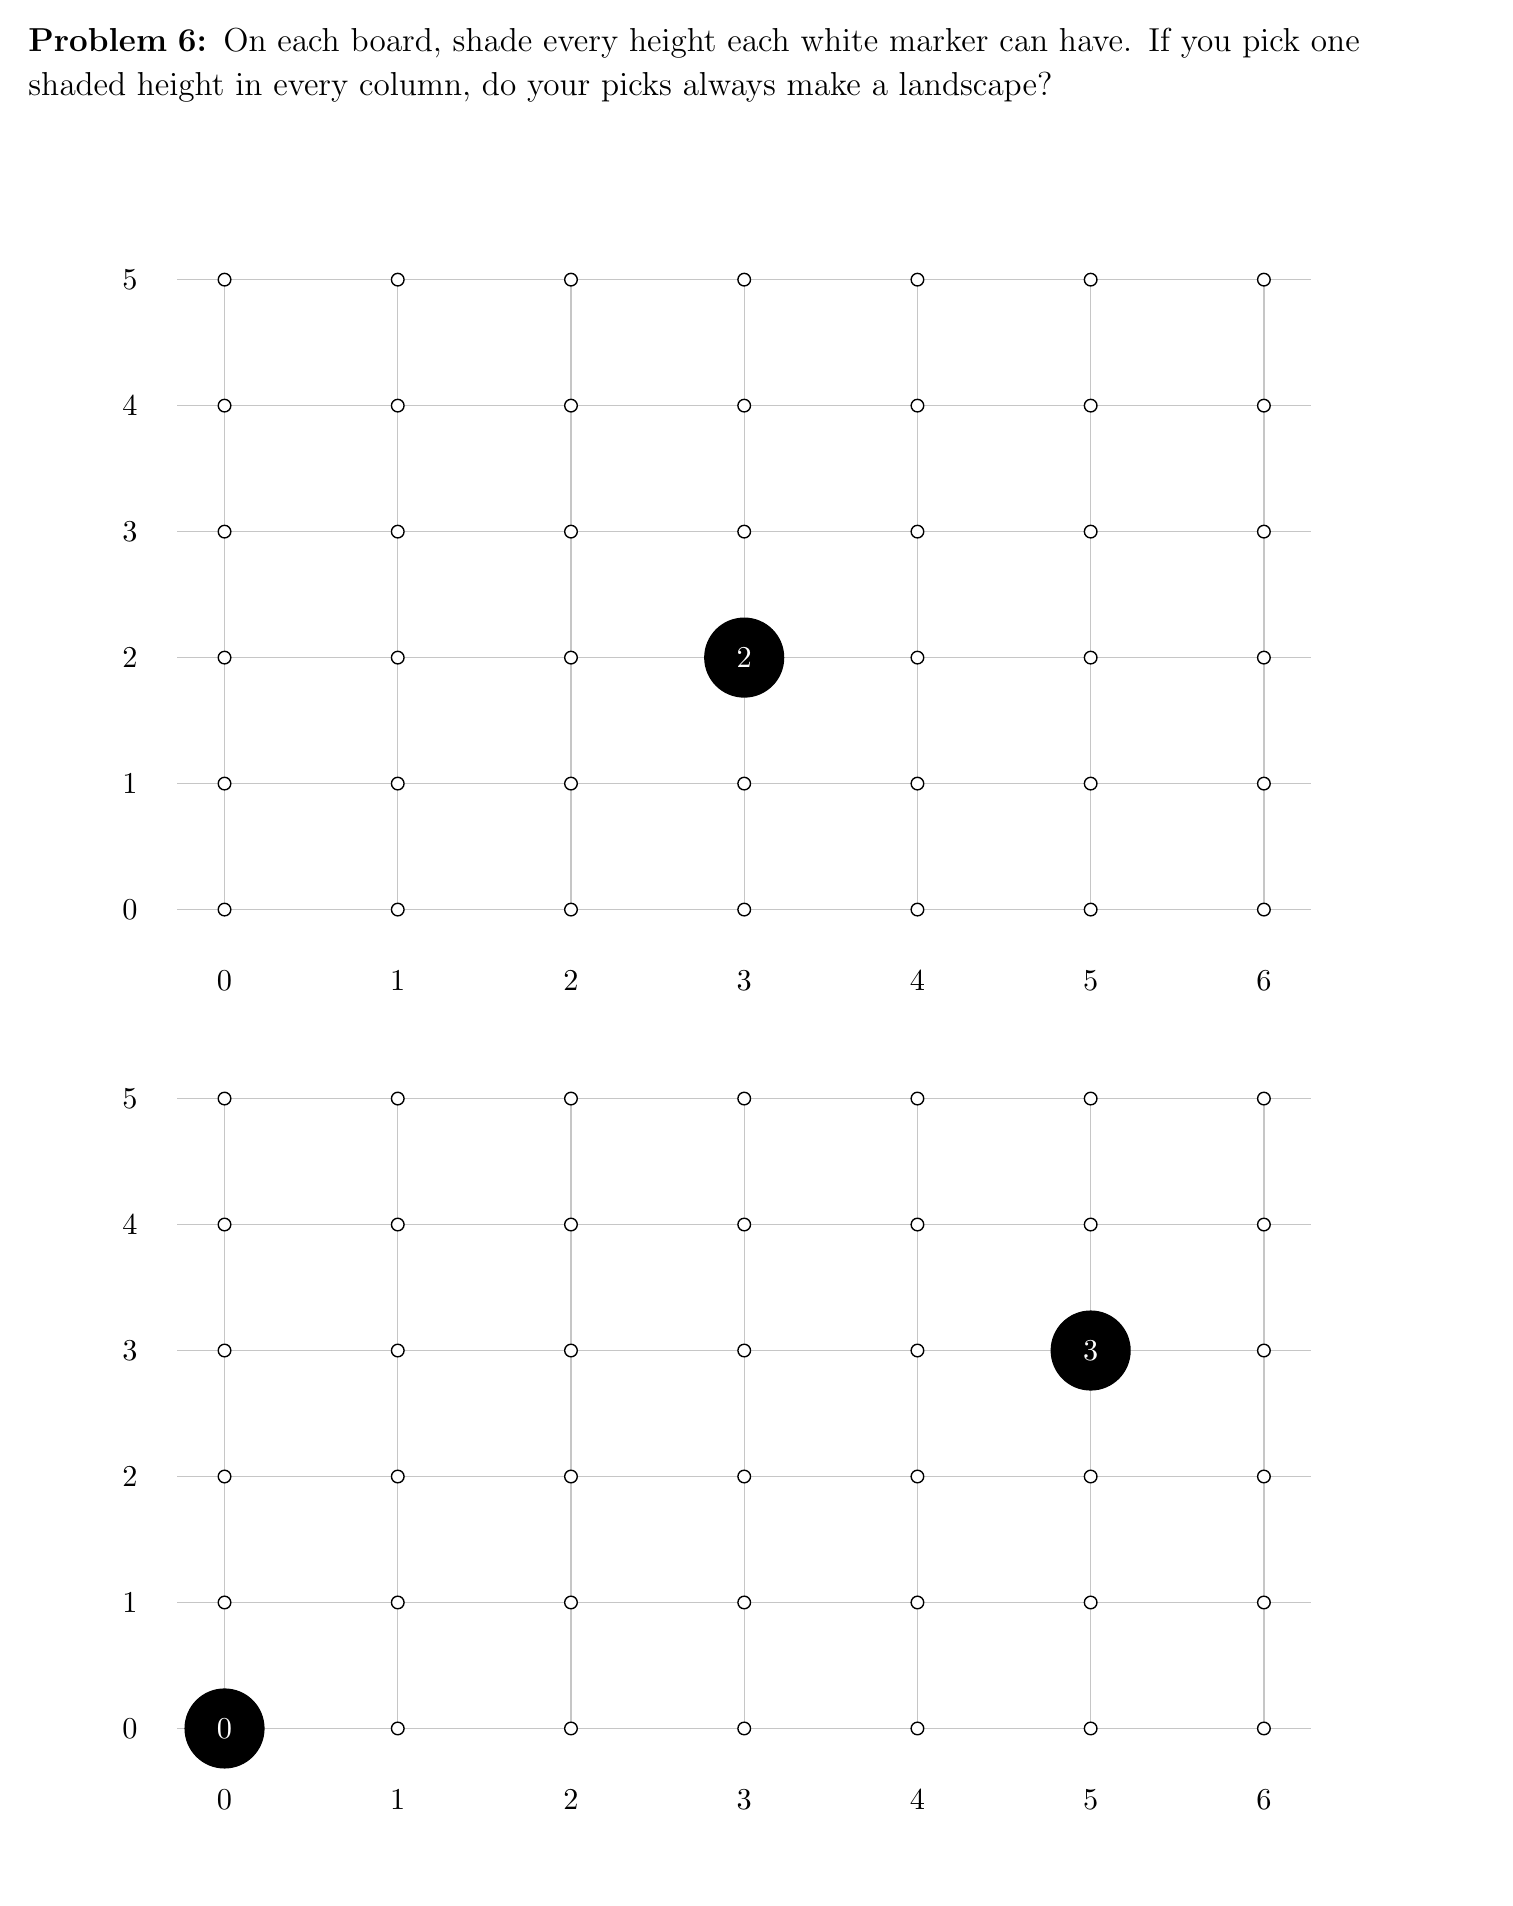
\begin{tikzpicture}[x=1mm,y=-1mm,line width=.5pt]
\path[use as bounding box] (0,0) rectangle (185,235);
\node[anchor=north west,inner sep=0pt,text width=180mm,font=\fontsize{13}{16}\selectfont] at (0,0) {\textbf{Problem 6:} On each board, shade every height each white marker can have. If you pick one shaded height in every column, do your picks always make a landscape?};
\draw[gray!45] (19,112) -- (163,112);
\node[anchor=center,inner sep=1pt,font=\fontsize{11}{13}\selectfont] at (13,112) {0};
\draw[gray!45] (19,96) -- (163,96);
\node[anchor=center,inner sep=1pt,font=\fontsize{11}{13}\selectfont] at (13,96) {1};
\draw[gray!45] (19,80) -- (163,80);
\node[anchor=center,inner sep=1pt,font=\fontsize{11}{13}\selectfont] at (13,80) {2};
\draw[gray!45] (19,64) -- (163,64);
\node[anchor=center,inner sep=1pt,font=\fontsize{11}{13}\selectfont] at (13,64) {3};
\draw[gray!45] (19,48) -- (163,48);
\node[anchor=center,inner sep=1pt,font=\fontsize{11}{13}\selectfont] at (13,48) {4};
\draw[gray!45] (19,32) -- (163,32);
\node[anchor=center,inner sep=1pt,font=\fontsize{11}{13}\selectfont] at (13,32) {5};
\draw[gray!45] (25,32) -- (25,112);
\draw[fill=white] (25,112) circle (0.8);
\draw[fill=white] (25,96) circle (0.8);
\draw[fill=white] (25,80) circle (0.8);
\draw[fill=white] (25,64) circle (0.8);
\draw[fill=white] (25,48) circle (0.8);
\draw[fill=white] (25,32) circle (0.8);
\node[anchor=center,inner sep=1pt,font=\fontsize{11}{13}\selectfont] at (25,121) {0};
\draw[gray!45] (47,32) -- (47,112);
\draw[fill=white] (47,112) circle (0.8);
\draw[fill=white] (47,96) circle (0.8);
\draw[fill=white] (47,80) circle (0.8);
\draw[fill=white] (47,64) circle (0.8);
\draw[fill=white] (47,48) circle (0.8);
\draw[fill=white] (47,32) circle (0.8);
\node[anchor=center,inner sep=1pt,font=\fontsize{11}{13}\selectfont] at (47,121) {1};
\draw[gray!45] (69,32) -- (69,112);
\draw[fill=white] (69,112) circle (0.8);
\draw[fill=white] (69,96) circle (0.8);
\draw[fill=white] (69,80) circle (0.8);
\draw[fill=white] (69,64) circle (0.8);
\draw[fill=white] (69,48) circle (0.8);
\draw[fill=white] (69,32) circle (0.8);
\node[anchor=center,inner sep=1pt,font=\fontsize{11}{13}\selectfont] at (69,121) {2};
\draw[gray!45] (91,32) -- (91,112);
\draw[fill=white] (91,112) circle (0.8);
\draw[fill=white] (91,96) circle (0.8);
\draw[fill=white] (91,80) circle (0.8);
\draw[fill=white] (91,64) circle (0.8);
\draw[fill=white] (91,48) circle (0.8);
\draw[fill=white] (91,32) circle (0.8);
\node[anchor=center,inner sep=1pt,font=\fontsize{11}{13}\selectfont] at (91,121) {3};
\draw[fill=black] (91,80) circle (5);
\node[anchor=center,inner sep=1pt,font=\fontsize{11}{13}\selectfont] at (91,80) {\color{white}2};
\draw[gray!45] (113,32) -- (113,112);
\draw[fill=white] (113,112) circle (0.8);
\draw[fill=white] (113,96) circle (0.8);
\draw[fill=white] (113,80) circle (0.8);
\draw[fill=white] (113,64) circle (0.8);
\draw[fill=white] (113,48) circle (0.8);
\draw[fill=white] (113,32) circle (0.8);
\node[anchor=center,inner sep=1pt,font=\fontsize{11}{13}\selectfont] at (113,121) {4};
\draw[gray!45] (135,32) -- (135,112);
\draw[fill=white] (135,112) circle (0.8);
\draw[fill=white] (135,96) circle (0.8);
\draw[fill=white] (135,80) circle (0.8);
\draw[fill=white] (135,64) circle (0.8);
\draw[fill=white] (135,48) circle (0.8);
\draw[fill=white] (135,32) circle (0.8);
\node[anchor=center,inner sep=1pt,font=\fontsize{11}{13}\selectfont] at (135,121) {5};
\draw[gray!45] (157,32) -- (157,112);
\draw[fill=white] (157,112) circle (0.8);
\draw[fill=white] (157,96) circle (0.8);
\draw[fill=white] (157,80) circle (0.8);
\draw[fill=white] (157,64) circle (0.8);
\draw[fill=white] (157,48) circle (0.8);
\draw[fill=white] (157,32) circle (0.8);
\node[anchor=center,inner sep=1pt,font=\fontsize{11}{13}\selectfont] at (157,121) {6};
\draw[gray!45] (19,216) -- (163,216);
\node[anchor=center,inner sep=1pt,font=\fontsize{11}{13}\selectfont] at (13,216) {0};
\draw[gray!45] (19,200) -- (163,200);
\node[anchor=center,inner sep=1pt,font=\fontsize{11}{13}\selectfont] at (13,200) {1};
\draw[gray!45] (19,184) -- (163,184);
\node[anchor=center,inner sep=1pt,font=\fontsize{11}{13}\selectfont] at (13,184) {2};
\draw[gray!45] (19,168) -- (163,168);
\node[anchor=center,inner sep=1pt,font=\fontsize{11}{13}\selectfont] at (13,168) {3};
\draw[gray!45] (19,152) -- (163,152);
\node[anchor=center,inner sep=1pt,font=\fontsize{11}{13}\selectfont] at (13,152) {4};
\draw[gray!45] (19,136) -- (163,136);
\node[anchor=center,inner sep=1pt,font=\fontsize{11}{13}\selectfont] at (13,136) {5};
\draw[gray!45] (25,136) -- (25,216);
\draw[fill=white] (25,216) circle (0.8);
\draw[fill=white] (25,200) circle (0.8);
\draw[fill=white] (25,184) circle (0.8);
\draw[fill=white] (25,168) circle (0.8);
\draw[fill=white] (25,152) circle (0.8);
\draw[fill=white] (25,136) circle (0.8);
\node[anchor=center,inner sep=1pt,font=\fontsize{11}{13}\selectfont] at (25,225) {0};
\draw[fill=black] (25,216) circle (5);
\node[anchor=center,inner sep=1pt,font=\fontsize{11}{13}\selectfont] at (25,216) {\color{white}0};
\draw[gray!45] (47,136) -- (47,216);
\draw[fill=white] (47,216) circle (0.8);
\draw[fill=white] (47,200) circle (0.8);
\draw[fill=white] (47,184) circle (0.8);
\draw[fill=white] (47,168) circle (0.8);
\draw[fill=white] (47,152) circle (0.8);
\draw[fill=white] (47,136) circle (0.8);
\node[anchor=center,inner sep=1pt,font=\fontsize{11}{13}\selectfont] at (47,225) {1};
\draw[gray!45] (69,136) -- (69,216);
\draw[fill=white] (69,216) circle (0.8);
\draw[fill=white] (69,200) circle (0.8);
\draw[fill=white] (69,184) circle (0.8);
\draw[fill=white] (69,168) circle (0.8);
\draw[fill=white] (69,152) circle (0.8);
\draw[fill=white] (69,136) circle (0.8);
\node[anchor=center,inner sep=1pt,font=\fontsize{11}{13}\selectfont] at (69,225) {2};
\draw[gray!45] (91,136) -- (91,216);
\draw[fill=white] (91,216) circle (0.8);
\draw[fill=white] (91,200) circle (0.8);
\draw[fill=white] (91,184) circle (0.8);
\draw[fill=white] (91,168) circle (0.8);
\draw[fill=white] (91,152) circle (0.8);
\draw[fill=white] (91,136) circle (0.8);
\node[anchor=center,inner sep=1pt,font=\fontsize{11}{13}\selectfont] at (91,225) {3};
\draw[gray!45] (113,136) -- (113,216);
\draw[fill=white] (113,216) circle (0.8);
\draw[fill=white] (113,200) circle (0.8);
\draw[fill=white] (113,184) circle (0.8);
\draw[fill=white] (113,168) circle (0.8);
\draw[fill=white] (113,152) circle (0.8);
\draw[fill=white] (113,136) circle (0.8);
\node[anchor=center,inner sep=1pt,font=\fontsize{11}{13}\selectfont] at (113,225) {4};
\draw[gray!45] (135,136) -- (135,216);
\draw[fill=white] (135,216) circle (0.8);
\draw[fill=white] (135,200) circle (0.8);
\draw[fill=white] (135,184) circle (0.8);
\draw[fill=white] (135,168) circle (0.8);
\draw[fill=white] (135,152) circle (0.8);
\draw[fill=white] (135,136) circle (0.8);
\node[anchor=center,inner sep=1pt,font=\fontsize{11}{13}\selectfont] at (135,225) {5};
\draw[fill=black] (135,168) circle (5);
\node[anchor=center,inner sep=1pt,font=\fontsize{11}{13}\selectfont] at (135,168) {\color{white}3};
\draw[gray!45] (157,136) -- (157,216);
\draw[fill=white] (157,216) circle (0.8);
\draw[fill=white] (157,200) circle (0.8);
\draw[fill=white] (157,184) circle (0.8);
\draw[fill=white] (157,168) circle (0.8);
\draw[fill=white] (157,152) circle (0.8);
\draw[fill=white] (157,136) circle (0.8);
\node[anchor=center,inner sep=1pt,font=\fontsize{11}{13}\selectfont] at (157,225) {6};
\end{tikzpicture}
\newpage
\noindent\begin{tikzpicture}[x=1mm,y=-1mm,line width=.5pt]
\path[use as bounding box] (0,0) rectangle (185,235);
\node[anchor=north west,inner sep=0pt,text width=180mm,font=\fontsize{13}{16}\selectfont] at (0,0) {\textbf{Problem 7:} A row has at least one clue. Suppose every pair of clues differs by no more than the steps between them. Must the whole row be fillable? Give a construction that always works, or a set of clues that defeats the claim.};
\draw[gray!45] (19,140) -- (163,140);
\node[anchor=center,inner sep=1pt,font=\fontsize{11}{13}\selectfont] at (13,140) {0};
\draw[gray!45] (19,120) -- (163,120);
\node[anchor=center,inner sep=1pt,font=\fontsize{11}{13}\selectfont] at (13,120) {1};
\draw[gray!45] (19,100) -- (163,100);
\node[anchor=center,inner sep=1pt,font=\fontsize{11}{13}\selectfont] at (13,100) {2};
\draw[gray!45] (19,80) -- (163,80);
\node[anchor=center,inner sep=1pt,font=\fontsize{11}{13}\selectfont] at (13,80) {3};
\draw[gray!45] (19,60) -- (163,60);
\node[anchor=center,inner sep=1pt,font=\fontsize{11}{13}\selectfont] at (13,60) {4};
\draw[gray!45] (19,40) -- (163,40);
\node[anchor=center,inner sep=1pt,font=\fontsize{11}{13}\selectfont] at (13,40) {5};
\draw[gray!45] (25,40) -- (25,140);
\draw[fill=white] (25,140) circle (0.8);
\draw[fill=white] (25,120) circle (0.8);
\draw[fill=white] (25,100) circle (0.8);
\draw[fill=white] (25,80) circle (0.8);
\draw[fill=white] (25,60) circle (0.8);
\draw[fill=white] (25,40) circle (0.8);
\node[anchor=center,inner sep=1pt,font=\fontsize{11}{13}\selectfont] at (25,149) {0};
\draw[gray!45] (47,40) -- (47,140);
\draw[fill=white] (47,140) circle (0.8);
\draw[fill=white] (47,120) circle (0.8);
\draw[fill=white] (47,100) circle (0.8);
\draw[fill=white] (47,80) circle (0.8);
\draw[fill=white] (47,60) circle (0.8);
\draw[fill=white] (47,40) circle (0.8);
\node[anchor=center,inner sep=1pt,font=\fontsize{11}{13}\selectfont] at (47,149) {1};
\draw[gray!45] (69,40) -- (69,140);
\draw[fill=white] (69,140) circle (0.8);
\draw[fill=white] (69,120) circle (0.8);
\draw[fill=white] (69,100) circle (0.8);
\draw[fill=white] (69,80) circle (0.8);
\draw[fill=white] (69,60) circle (0.8);
\draw[fill=white] (69,40) circle (0.8);
\node[anchor=center,inner sep=1pt,font=\fontsize{11}{13}\selectfont] at (69,149) {2};
\draw[gray!45] (91,40) -- (91,140);
\draw[fill=white] (91,140) circle (0.8);
\draw[fill=white] (91,120) circle (0.8);
\draw[fill=white] (91,100) circle (0.8);
\draw[fill=white] (91,80) circle (0.8);
\draw[fill=white] (91,60) circle (0.8);
\draw[fill=white] (91,40) circle (0.8);
\node[anchor=center,inner sep=1pt,font=\fontsize{11}{13}\selectfont] at (91,149) {3};
\draw[gray!45] (113,40) -- (113,140);
\draw[fill=white] (113,140) circle (0.8);
\draw[fill=white] (113,120) circle (0.8);
\draw[fill=white] (113,100) circle (0.8);
\draw[fill=white] (113,80) circle (0.8);
\draw[fill=white] (113,60) circle (0.8);
\draw[fill=white] (113,40) circle (0.8);
\node[anchor=center,inner sep=1pt,font=\fontsize{11}{13}\selectfont] at (113,149) {4};
\draw[gray!45] (135,40) -- (135,140);
\draw[fill=white] (135,140) circle (0.8);
\draw[fill=white] (135,120) circle (0.8);
\draw[fill=white] (135,100) circle (0.8);
\draw[fill=white] (135,80) circle (0.8);
\draw[fill=white] (135,60) circle (0.8);
\draw[fill=white] (135,40) circle (0.8);
\node[anchor=center,inner sep=1pt,font=\fontsize{11}{13}\selectfont] at (135,149) {5};
\draw[gray!45] (157,40) -- (157,140);
\draw[fill=white] (157,140) circle (0.8);
\draw[fill=white] (157,120) circle (0.8);
\draw[fill=white] (157,100) circle (0.8);
\draw[fill=white] (157,80) circle (0.8);
\draw[fill=white] (157,60) circle (0.8);
\draw[fill=white] (157,40) circle (0.8);
\node[anchor=center,inner sep=1pt,font=\fontsize{11}{13}\selectfont] at (157,149) {6};
\end{tikzpicture}
\end{document}
